% Two overlapping sets: outlines encode membership, not adjacent-panel proxies.
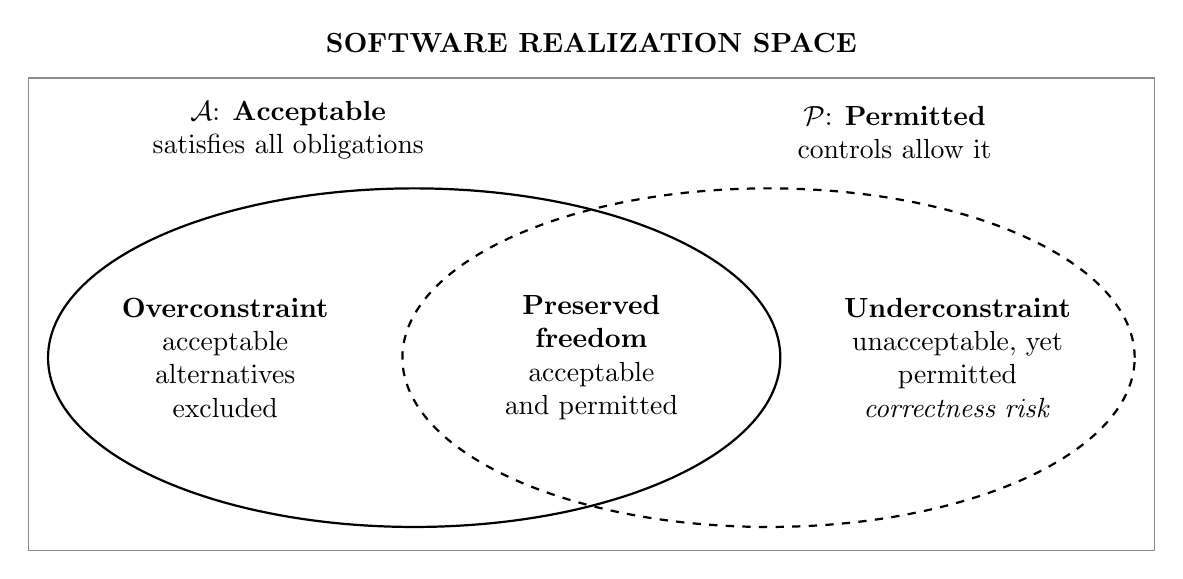
\begin{tikzpicture}[x=1cm,y=1cm,
 font=\magefigurefont\fontsize{10}{12}\selectfont,
 every node/.style={align=center,inner sep=2pt,text=black,
 execute at begin node={\hyphenpenalty=10000\exhyphenpenalty=10000}}]
\node[font=\magefigurefont\fontsize{10}{12}\selectfont\bfseries]
 at (7.05,.9) {SOFTWARE REALIZATION SPACE};
\draw[black!45,line width=.5pt] (-.1,.45) rectangle (14.2,-5.55);
\node[anchor=south] at (3.2,-.65) {$\mathcal A$: \textbf{Acceptable}\\satisfies all obligations};
\node[anchor=south] at (10.9,-.65) {$\mathcal P$: \textbf{Permitted}\\controls allow it};
\draw[line width=.8pt] (4.8,-3.1) ellipse [x radius=4.65cm,y radius=2.15cm];
\draw[dashed,line width=.8pt] (9.3,-3.1) ellipse [x radius=4.65cm,y radius=2.15cm];
\node[text width=3.1cm] at (2.4,-3.1) {\textbf{Overconstraint}\\acceptable alternatives\\excluded};
\node[text width=3cm] at (7.05,-3.1) {\textbf{Preserved freedom}\\acceptable\\and permitted};
\node[text width=3.3cm] at (11.7,-3.1) {\textbf{Underconstraint}\\unacceptable, yet\\permitted\\\textit{correctness risk}};
\end{tikzpicture}
